\newcommand{\sig}{\sigma}
\newcommand{\Sig}{\Sigma}
\newcommand{\eps}{\epsilon}
\newcommand{\del}{\delta}
\newcommand{\ah}{\alpha}
\newcommand{\lam}{\lambda}
\newcommand{\gam}{\gamma}
\newcommand{\kap}{\kappa}
\newcommand{\rarr}{\rightarrow}
\newcommand{\larr}{\leftarrow}
\newcommand{\Rarr}{\Rightarrow}
\newcommand{\Larr}{\Leftarrow}

\newcommand{\ol}{\overline}
\newcommand{\dagg}{\dagger}
\newcommand{\mbb}{\mathbb}
\newcommand{\contra}{\Rightarrow\Leftarrow}
% for cross product
\newcommand{\lc}{\langle} %<
\newcommand{\rc}{\rangle} %>
% linear alg
\newcommand{\inv}{^{-1}}
\renewcommand{\vec}[1]{\boldsymbol{#1}}
\newcommand{\kth}{^{(k)}}
% order 
\newcommand{\cO}{\mathcal{O}}
% gradient
\newcommand{\grad}{\nabla}
\newcommand{\ddx}{\frac \partial {\partial x}}

%other shortcuts
\newcommand{\ben}{\begin{enumerate}}
\newcommand{\een}{\end{enumerate}}
\newcommand{\beq}{\begin{quote}}
\newcommand{\enq}{\end{quote}}
\newcommand{\hsone}{\hspace*{1cm}}
\newcommand{\hstwo}{\hspace*{2cm}}

\newcommand{\noi}{\noindent}
\parskip 5pt
\parindent 0pt

\documentclass[a4paper]{article}
\usepackage{amsmath,amssymb,hyperref,graphicx}
\begin{document}
\title{Affine Structure from Motion}
\author{Scientific Computing CS660 Fall '11 Final Project \\ Angjoo Kanazawa}
\date{\today}
\maketitle

\section{Introduction}
Over the last few decades, the influence of Scientific Computing has
been so prevelent in almost every area of Science and Engineering. It has
become a necessary and critical tool for anyone involved in high-level
research in Computer Science. Computer Vision is one of the quintessential example of a research area that heavily builds upon
methods discovered in Scientific Computing, where the primary interest
lies in the analysis and understanding of images which are represented
in numerical matrices. This project explores applications of
computational algorithms explored in Scientific Computing via tackling
the problem of 3D reconstruction of an object from a stream of images.

The 3D reconstruction problem consists of a series of challenges starting from developing the
cameral model and feature representation of the image,
tracking such features over the image sequences , and finally
reconstructing the 3D geometry from the tracked points. In all of these steps,  The application of algorithms explored in
Scientific Computing is ubiqutous in all of these steps. 

The main challenge of recovering 3D geometry of objects and camera motion simultaneously from a set of point
correspondences is referred to as the Structure from Motion (SfM) problem. The solution to the problem has a
wide range of application in 3D modelling, virtual and augmented
reality models in computer graphics, camera calibration and many
more. It is a well studied problem with various approaches; this project focuses on the \emph{factorization} method proposed by Tomasi and Kanade
\cite{Tomasi} under the orthographic camera projection model. The
algorithm provides a numerically stable closed from optimal solution
via the singular-value decomposition technique under certain
conditions. \cite[p. 435]{AZ}

This project follows the Project 4 of Derek Hoiem's CS 543/ECE 549
course at the University of Illinois at Urbana-Champaign:
\href{http://www.cs.illinois.edu/class/sp11/cs543/hw/hw4.pdf}{project
  description}. 

\section{Background}

\subsection{Orthographic Projection}
\label{sec:ortho}
A camera model transforms a world point into an
image point. An affine camera, often used for
its simplicity, preserves up to affine transformation of world points
to image points. Basically it is a linear mapping followed by a translation, where
points can rotate, scale, and translate but parallelism is
preserved.\cite[p.38]{Szelski}. 
% \begin{figure}[!ht]
%   \begin{center}
%   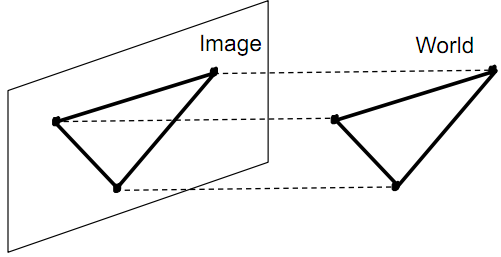
\includegraphics[scale=0.6]{ortho.png}
%   \caption{Orthographic Projection} 
%   \label{figures:ortho}
%   \end{center}
% \end{figure}
An \emph{orthographic
camera model} is a specific type of affine camera where the world
points are projected in parallel onto the image plane, where the depth
information of the world $Z$, is simply ignored. Mathematically, 
\begin{align*}
\begin{pmatrix}
  x\\y
\end{pmatrix} &= \begin{pmatrix}
  1& 0&0 \\0 & 1 & 0
\end{pmatrix}
R
\begin{pmatrix}
  X\\Y\\Z\\
\end{pmatrix} + \vec t\\
\vec x = P\vec X + \vec t
\end{align*}
Where $P = \begin{smallmatrix}
  1& 0&0 \\0 & 1 & 0
\end{smallmatrix}R$ is referred to as the projection matrix, and $R$
is a 3 by 3 matrix representing the affine motion (rotation, translation, or
both) of the camrea and $t$ is the displacement vector \cite[p.172]{AZ}. 

\subsection{Notations and Assumptions}
\label{sec:notations}
A ``world point'' refers to a point, in the 3D
coordinate system, $\vec X = (X,Y,Z)^T$, and an ``image point'' refers
to a point projected on to an image plane in the 2D coordinate system,
$\vec x =(x,y)^T$. 

$I(x,y)$ denotes the pixel intensity value of image $I$, and $I(x,y,t)$ denotes the
pixel value of image $I$ at time $t$. $\grad I$ is the image gradient
$[I_x  I_y]$ and $H$ is the image hessian $\begin{smallmatrix}  I_x^2
  & I_xI_y \\ I_yI_x & I_y^2\end{smallmatrix}$

In this project, all projection is orthographic \ref{sec:ortho}
and camera motion is affine. The world projected on the image
sequences is rigid and the pixel intensities of images over sequences are
constant i.e. all frames taken under static environment with no
brightness changes. Also for the experiment we assume that there is
no occlusion.

\subsection{Problem Statement}
\label{sec:problem-statement}
Given $F$ frames of sequencial images (videos), obtain $P$ trajectory
of image points for all $F$: $\{x_{fp} = (u_{fp}, v_{fp})^T
\forall F, P$ and solve for $X_{p}$, the world coordinate of all $P$ points.
these observation. 

\section{Structure for Motion}
\label{sec:main}
There are three main components for 3D reconstruction of an image stream. First we need to select a subset of
``interesting'' pixels from the original frame. These points are then
tracked through out the rest of the squence. This set of point
correspondence across all frames is then fed into the factorization algorithm. Appropriate keypoint selection and accurate feature tracking
are critical for a successful 3D reconstruction. 

\subsection{Keypoint Selection}
\label{sec:keypoint-selection}
It's not computationally possible to solve the world coordinate for every pixel of image sequences. We need to
select keypoints in the image that are distinct, reliable and
meaningful. 

\emph{Harris corner detector} is an optimal feature selection for the
tracker that is used for this project. (It's optimality is discussed
in section \ref{sec:feature-tracking}). The idea is that we should easily recognize an interesting point by looking through a
small window, where shifting a window in any direction
should give a large change in intensity i.e. we accept a point $\vec x$ if SSD of
the displacement of the window by $(u,v)^T$, $E(u,v) =
\sum_{(x,y)\in W} [I(x+u, y+v) - I(x,y)]^2$, is large in all
direction. 
Assuming $\vec d = (u,v)^T$ is small, the taylor series expansion of $I$ is
$$I(x+u, y+v) \approx I(x,y) + I_xu +I_yv + \cO(d^Td)$$ where $I_x
=\frac{\partial I}{\partial x} $, $I_y = \frac{\partial I}{\partial y}$.

Then, 
\begin{align*}
  E(u,v) &=\sum_{(x,y)\in W} [I(x+u, y+v) - I(x,y)]^2\\
&=\sum_{(x,y)\in W} [I(x,y) + I_xu +
I_yv - I(x,y)]^2\\
&= \sum_{(x,y)\in W} (
\begin{pmatrix}
  I_x & I_y
\end{pmatrix}
\cdot
\begin{pmatrix}
  u \\ v
\end{pmatrix}
)^2\\
&= \begin{pmatrix}
  u & v
\end{pmatrix} 
\begin{pmatrix}  I_x^2
  & I_xI_y \\ I_yI_x & I_y^2\end{pmatrix} \begin{pmatrix}
  u \\ v
\end{pmatrix}\\
&=d^T H d.
\end{align*}
  Since the two eigenvalues of $H$
,$\lam_1, \lam_2$, denotes the amount of change in the direction of its corresponding
eigenvector, we accept a window if $min(\lam_1, \lam_2) > \tau$, where
$\tau$ is predefined threshold \cite{shi}. Figure \ref{fig:Hessian} illustrates
the components of the Hessisan of frame one. 

% \begin{figure}[!ht]
%   \begin{center}
%   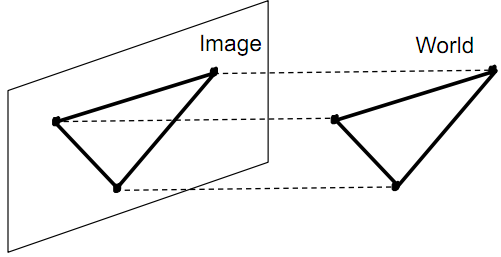
\includegraphics[scale=0.5]{ortho.png}
%   \caption{Plot of the image gradients of the first frame} 
%   \label{fig:Hessian}
%   \end{center}
% \end{figure}

\subsection{Feature Tracking}
\label{sec:feature-tracking}
Now using the detected keypoint, we track these points over all frames
using the Kanade-Lucas-Tomasi (KLT) Tracker \cite{KLT}.
The basis of KLT tracker is that although image intensities change as
camera moves, images taken at near time are strongly related to each
other because they tend to refer to the same scene given the
assumption of local brightness constancy. This means that under an ideal
static environment, image at time $t+1$ can be obtained by moving
every pixel in the at time image $t$ by a suitable amount \cite{shi}. 

\subsubsection{Estimating Camera Motion}
This displacement can be either a translation or an affine mapping or
the combination of both, but since the world is rigid we will only
consider translation. Mathematically, given $\vec x$ at frame $t$, we
want to find a displacement vector, $\vec d=(u,v)^T$, that minimizes
the dissimilarity
\begin{equation}
  \label{eq:1}
 I(\vec x + \vec d, t+1) - I(\vec x, t) = 0
\end{equation}

The taylor expansion of $$I(\vec x+\vec d, t+1) = I(x+u, y+v, t+1) \approx I(x,y,t) + I_xu +
I_yv + I(x+u, y+u, t) + I_t \cO(d^Td).$$  Where $I_t$ is the temporal
gradient (for time) $I_t(\vec x) =I(\vec x, t) - I(\vec x+\vec d, t+1)$. Substituting that back to \eqref{eq:1},
\begin{align*}
0 &\approx I(x,y,t) + I_xu +I_yv  + I_t - I(x,y,t)\\
&= \grad I(\vec x)\cdot \vec d + I_t(\vec x)
\end{align*}
 Here we have 2
unknowns but only one constraint. In fact even with the brightness
constancy assumption, it is difficult to track a single point unless
the point is extremely distinctive \cite{KLT}. Therefore we consider minimizing
the dissimilarity within a small window (typically around 15 x 15) and
obtain an overdetermined linear system of equations:
\begin{align*}
\sum_{\vec x\in W} \grad I(\vec x) \cdot \vec d &= \sum_{\vec x\in W}
I_t \\
A\vec d &= \vec t
\end{align*}
Using the normal equations, we solve this least linear squares
problem:

\begin{align}  \label{eq:klt}
  A^TA\vec d &= A^T \vec t\\
  \begin{pmatrix}
    I_x(x_1) & \hdots & I_x(x_{|W|}) \\
   \vdots &  & \vdots \\
  I_y(x_1) & \hdots & I_y(x_{|W|}) \\
  \end{pmatrix}
  \begin{pmatrix}
    I_x(x_1) & \hdots &   I_y(x_1)  \\
   \vdots &  & \vdots \\
I_x(x_{|W|})& \hdots & I_y(x_{|W|}) \\
  \end{pmatrix}
\vec d  &= 
  \begin{pmatrix}
    I_x(x_1) & \hdots &   I_y(x_1)  \\
   \vdots &  & \vdots \\
I_x(x_{|W|})& \hdots & I_y(x_{|W|}) \\
  \end{pmatrix}
  \begin{pmatrix}
    I_t(x_1)\\ \vdots \\ I_t(x_{|w|})
  \end{pmatrix}\\
\begin{pmatrix}
\sum_{\vec x\in W}  I_x^2 &\sum_{\vec x\in W} I_xI_y\\ \sum_{\vec x\in
  W} I_y^2 &\sum_{\vec x\in W} I_yI_x
\end{pmatrix}
\begin{pmatrix}
  u \\ v
\end{pmatrix}
 &=
\begin{pmatrix}
 \sum_{\vec x\in W} I_xI_t\\ \sum_{\vec x\in W}I_yI_t
\end{pmatrix} \\
Z\vec d &= \vec e
\end{align}

Since solving for $\vec d$ by the method above requires us to konw
$I_t$, which requires an initial displacement $\vec d_0$, so we solve
for the verctor iteratively. Namely, we start with $\vec d_0
=(0,0)^T$ to compute $I_{t_0} = I(\vec x, t+1) - I(\vec x, t)$, then
solve for $\vec d_1$ using $I_{t_0}$. We iterate this until $||\vec
d_k - \vec d_{k+1}|| \le \delta$, $\delta$ some threshold.

\subsubsection{Numerical Stability}
\label{sec:numerical-stability}
Can we solve \eqref{eq:4} reliably? It seems like in practice, it's
not unusual to solve for $\vec d$ simply by taking the pseudo-inverse of $Z$,
which is known to be atrocious in the Scientific Computing
community. But there is a reason why here it is okay to be less
careful about solving for $\vec d$ and it leads to the discussion of
the optimality of our key point selecter.

For \eqref{eq:4} to be stable, w need $Z$ to be
well-conditioned. The condition number of $Z$ is $\kappa(Z) =
||A||||A\inv||$. Here, $Z$ is symmetric and positive definite (because
it's the Hessian), so the condition number is also the ratio of the
smallest to largest eigenvalue. Here it's $\frac{\lam_1}{\lam_2}$.
Note that our criteria for choosing our keypoint was $\min(\lam_1,
\lam_2) > \tau$. So we are assured that $\lam_2$ eigenvalue is
sufficiently large. Since we're dealing with images with a maximum
possible pixel value, we are also assured that $\lam_1$ will not be
arbitrarily large. So with this keypoint selection, we're guaranteed to
have a well conditioned $Z$. This is why in practice it is okay to use the pseudo-inverse
of $Z$. This means in MATLAB the \texttt{mldivide} is more than
sufficient.


\subsection{The Factorization Method}
As discussed in \ref{sec:ortho}, orthographic camera model projects
the world points onto the image plane as a linear mapping followed by
a translation $x = PX + t$. Using the set of tracked corresponding
points, we can represent the image sequence by a $2F\times P$ \emph{measurement matrix
}$W$, where $w_{fp} = (x_{fp}, y_{fp})^T$, and
$P$ is the number of points tracked through $F$
frames.   

To get rid of the translation term, we center the image points by
subtracting the mean (centroid) of image points, and assume that
the world coordinate system is at the centroid of the 3D points. Then,
the orientation (rotation) of the camera at frame $f$ is represented by orthonormal
vectors $i_f, j_f, k_f \in \mathbf{R}^{3}$, where each vector
corresponds to the x, y, and z-axis of the image plane
respectively. Under orthography with the $z$ axis along the optical
axis, these vectors over $F$ frames are collected into a
\emph{motion matrix} $M\in \mathbf{R}^{2F \times 3}$ $$M =
\begin{pmatrix}
  i_1^T\\ \vdots \\  i_F^T \\ j_1^T \\ \vdots j_F^T
\end{pmatrix}
$$
We let $S_p = (X_p, Y_p, Z_p)^T$ be the 3D coordinates of feature $p$ in the fixed world point with the same origin. These vectors are collected into a
\emph{shape matrix} $S\in \mathbf{R}^{3 \times P}$ s.t. $S =
\begin{pmatrix}
  s_1 & \cdots & s_p
\end{pmatrix}^T$. Using this notation, for a single frame we get
\begin{align*}
  \begin{pmatrix}
    x_{fp}\\y_{fp}
  \end{pmatrix} &=
  \begin{pmatrix}
    i_{f}^T\\j_{f}^T
  \end{pmatrix}
  \begin{pmatrix}
    X_p\\ Y_p\\ Z_p
  \end{pmatrix}\\
w_{fp} &= M_fS_p  
\end{align*}

So for all frames, we have the equation $$W = MS$$
Our goal is to estimate $\hat M$ and $\hat S$, s.t. $\hat W = \hat M
\hat S$, our estimated
measurement matrix, and the actual $W$ is minimized i.e. $$\min_{M,
  S}||W- \hat M \hat S||^2$$
a least squares problem.
\cite{Tomasi} proved that under this model, the rank of $W$ is 3. So
we can achieve the least squares approximation by factoring $W$ by
SVD. Namely, 
\begin{align*}
W &= U\Sigma V^T\\
&\approx U_3\tilde \Sigma V_3^T \text{ because $W$ is rank 3}\\
&=
\begin{pmatrix}
  u_{1,1} & u_{1,2} & u_{1,3} \\ \vdots & & \vdots
\\ \vdots & & \vdots
\\   u_{2F,1} & u_{2F,2} & u_{2F,3} 
\end{pmatrix}
\begin{pmatrix}
  \sigma_1 & 0 & 0 \\
  0 & \sigma_2 & 0 \\
  0 & 0 & \sigma_3 \\
\end{pmatrix}
\begin{pmatrix}
  v_{1,1} &  \cdots &\cdots & v_{1,p}\\
  v_{2,1} &  \cdots &\cdots & v_{2,p}\\
  v_{3,1} &  \cdots &\cdots & v_{3,p}\\
\end{pmatrix}
\end{align*}

Where possible solution is to choose $\hat M = U_3\tilde \Sigma^{1/2}$
and $\hat S =\tilde \Sigma^{1/2}V_3^T$. This solution can be refined
by eliminating affine ambiguity, but this algorithm is numerically
stable and it is guaranteed to converge to the global minimum of the
least squares problem.

\section{Eliminating Affine Ambiguity}



\section{Results and Analysis}
\label{sec:results}


\section{Conclusion}
\label{sec:conclusion}

\bibliographystyle{plain}
\bibliography{reference}
\end{document}
